\documentclass[twoside]{book}

% Packages required by doxygen
\usepackage{calc}
\usepackage{doxygen}
\usepackage{graphicx}
\usepackage[utf8]{inputenc}
\usepackage{makeidx}
\usepackage{multicol}
\usepackage{multirow}
\usepackage{textcomp}
\usepackage[table]{xcolor}

% Font selection
\usepackage[T1]{fontenc}
\usepackage{mathptmx}
\usepackage[scaled=.90]{helvet}
\usepackage{courier}
\usepackage{amssymb}
\usepackage{sectsty}
\renewcommand{\familydefault}{\sfdefault}
\allsectionsfont{%
  \fontseries{bc}\selectfont%
  \color{darkgray}%
}
\renewcommand{\DoxyLabelFont}{%
  \fontseries{bc}\selectfont%
  \color{darkgray}%
}

% Page & text layout
\usepackage{geometry}
\geometry{%
  a4paper,%
  top=2.5cm,%
  bottom=2.5cm,%
  left=2.5cm,%
  right=2.5cm%
}
\tolerance=750
\hfuzz=15pt
\hbadness=750
\setlength{\emergencystretch}{15pt}
\setlength{\parindent}{0cm}
\setlength{\parskip}{0.2cm}
\makeatletter
\renewcommand{\paragraph}{%
  \@startsection{paragraph}{4}{0ex}{-1.0ex}{1.0ex}{%
    \normalfont\normalsize\bfseries\SS@parafont%
  }%
}
\renewcommand{\subparagraph}{%
  \@startsection{subparagraph}{5}{0ex}{-1.0ex}{1.0ex}{%
    \normalfont\normalsize\bfseries\SS@subparafont%
  }%
}
\makeatother

% Headers & footers
\usepackage{fancyhdr}
\pagestyle{fancyplain}
\fancyhead[LE]{\fancyplain{}{\bfseries\thepage}}
\fancyhead[CE]{\fancyplain{}{}}
\fancyhead[RE]{\fancyplain{}{\bfseries\leftmark}}
\fancyhead[LO]{\fancyplain{}{\bfseries\rightmark}}
\fancyhead[CO]{\fancyplain{}{}}
\fancyhead[RO]{\fancyplain{}{\bfseries\thepage}}
\fancyfoot[LE]{\fancyplain{}{}}
\fancyfoot[CE]{\fancyplain{}{}}
\fancyfoot[RE]{\fancyplain{}{\bfseries\scriptsize Generated on Fri May 31 2019 14\-:03\-:56 for Tool\-D\-A\-Q\-Framework by Doxygen }}
\fancyfoot[LO]{\fancyplain{}{\bfseries\scriptsize Generated on Fri May 31 2019 14\-:03\-:56 for Tool\-D\-A\-Q\-Framework by Doxygen }}
\fancyfoot[CO]{\fancyplain{}{}}
\fancyfoot[RO]{\fancyplain{}{}}
\renewcommand{\footrulewidth}{0.4pt}
\renewcommand{\chaptermark}[1]{%
  \markboth{#1}{}%
}
\renewcommand{\sectionmark}[1]{%
  \markright{\thesection\ #1}%
}

% Indices & bibliography
\usepackage{natbib}
\usepackage[titles]{tocloft}
\setcounter{tocdepth}{3}
\setcounter{secnumdepth}{5}
\makeindex

% Hyperlinks (required, but should be loaded last)
\usepackage{ifpdf}
\ifpdf
  \usepackage[pdftex,pagebackref=true]{hyperref}
\else
  \usepackage[ps2pdf,pagebackref=true]{hyperref}
\fi
\hypersetup{%
  colorlinks=true,%
  linkcolor=blue,%
  citecolor=blue,%
  unicode%
}

% Custom commands
\newcommand{\clearemptydoublepage}{%
  \newpage{\pagestyle{empty}\cleardoublepage}%
}


%===== C O N T E N T S =====

\begin{document}

% Titlepage & ToC
\hypersetup{pageanchor=false}
\pagenumbering{roman}
\begin{titlepage}
\vspace*{7cm}
\begin{center}%
{\Large Tool\-D\-A\-Q\-Framework }\\
\vspace*{1cm}
{\large Generated by Doxygen 1.8.5}\\
\vspace*{0.5cm}
{\small Fri May 31 2019 14:03:56}\\
\end{center}
\end{titlepage}
\clearemptydoublepage
\tableofcontents
\clearemptydoublepage
\pagenumbering{arabic}
\hypersetup{pageanchor=true}

%--- Begin generated contents ---
\chapter{Configure files}
\label{md_configfiles_README}
\hypertarget{md_configfiles_README}{}


 \#\-Description 



Configure files are simple text files for passing variables to the Tools.

Text files are read by the \hyperlink{classStore}{Store} class (src/\-Store) and automatically asigned to an internal map for the relavent \hyperlink{classTool}{Tool} to use.



 \#\-Useage 



Any line starting with a \char`\"{}\#\char`\"{} will be ignored by the \hyperlink{classStore}{Store}, as will blank lines.

Variables should be stored one per line as follows\-:

Name Value \#\-Comments

Note\-: Only one value is permitted per name and they are stored in a string stream and templated cast back to the type given. 
\chapter{Configure files}
\label{md_configfiles_template_README}
\hypertarget{md_configfiles_template_README}{}


 \#\-Description 



Configure files are simple text files for passing variables to the Tools.

Text files are read by the \hyperlink{classStore}{Store} class (src/\-Store) and automatically asigned to an internal map for the relavent \hyperlink{classTool}{Tool} to use.



 \#\-Useage 



Any line starting with a \char`\"{}\#\char`\"{} will be ignored by the \hyperlink{classStore}{Store}, as will blank lines.

Variables should be stored one per line as follows\-:

Name Value \#\-Comments

Note\-: Only one value is permitted per name and they are stored in a string stream and templated cast back to the type given. 
\chapter{R\-E\-A\-D\-M\-E}
\label{md_DataModel_README}
\hypertarget{md_DataModel_README}{}
\#\-Data Model 



Data Model Class can be defined how ever the User requires. A \hyperlink{classStore}{Store} is provided which ineficently maps variables to string lkeys via conversion to stringstream and can be used for debuging or other useful vairables.

A T\-Tree map with getter and setter functions is provided and can be uncommented if required. 
\chapter{D\-A\-Q\-Framework}
\label{md_include_README}
\hypertarget{md_include_README}{}
\input{md_include_README}
\chapter{D\-A\-Q\-Framework}
\label{md_lib_README}
\hypertarget{md_lib_README}{}
\input{md_lib_README}
\chapter{Tool\-D\-A\-Q Framework}
\label{md_README}
\hypertarget{md_README}{}
Tool\-D\-A\-Q is an open source general modular D\-A\-Q Frame\-Work, with built in service discovery.



 \#\-Concept 



The main executable creates a \hyperlink{classToolChain}{Tool\-Chain} which is an object that holds Tools. Tools are added to the \hyperlink{classToolChain}{Tool\-Chain} and then the \hyperlink{classToolChain}{Tool\-Chain} can be told to Initialise Execute and Finalise each tool in the chain.

The \hyperlink{classToolChain}{Tool\-Chain} also holds a uesr defined \hyperlink{classDataModel}{Data\-Model} which each tool has access too and can read ,update and modify. This is the method by which data is passed between Tools.

User Tools can be generated for use in the tool chain by incuding a \hyperlink{classTool}{Tool} header. This can be done manually or by use of the new\-Tool.\-sh script.

For more information consult the Tool\-D\-A\-Q doc.\-pdf

\href{https://github.com/ToolDAQ/ToolDAQFramework/blob/master/ToolDAQ%20doc.pdf}{\tt https\-://github.\-com/\-Tool\-D\-A\-Q/\-Tool\-D\-A\-Q\-Framework/blob/master/\-Tool\-D\-A\-Q\%20doc.\-pdf}

Copyright (c) 2016 Benjamin Richards 
\chapter{D\-A\-Q\-Framework}
\label{md_src_Store_README}
\hypertarget{md_src_Store_README}{}
\input{md_src_Store_README}
\chapter{D\-A\-Q\-Framework}
\label{md_src_Tool_README}
\hypertarget{md_src_Tool_README}{}
\input{md_src_Tool_README}
\chapter{D\-A\-Q\-Framework}
\label{md_src_ToolChain_README}
\hypertarget{md_src_ToolChain_README}{}
\input{md_src_ToolChain_README}
\chapter{D\-A\-Q\-Framework}
\label{md_UserTools_README}
\hypertarget{md_UserTools_README}{}
\input{md_UserTools_README}
\chapter{D\-A\-Q\-Framework}
\label{md_UserTools_template_README}
\hypertarget{md_UserTools_template_README}{}
\input{md_UserTools_template_README}
\chapter{Hierarchical Index}
\section{Class Hierarchy}
This inheritance list is sorted roughly, but not completely, alphabetically\-:\begin{DoxyCompactList}
\item \contentsline{section}{Boost\-Store}{\pageref{classBoostStore}}{}
\item \contentsline{section}{Data\-Model}{\pageref{classDataModel}}{}
\item \contentsline{section}{Logging\-\_\-thread\-\_\-args}{\pageref{structLogging__thread__args}}{}
\item ostream\begin{DoxyCompactList}
\item \contentsline{section}{Logging}{\pageref{classLogging}}{}
\end{DoxyCompactList}
\item \contentsline{section}{Pointer\-Wrapper\-Base}{\pageref{classPointerWrapperBase}}{}
\begin{DoxyCompactList}
\item \contentsline{section}{Pointer\-Wrapper$<$ T $>$}{\pageref{classPointerWrapper}}{}
\end{DoxyCompactList}
\item \contentsline{section}{Serialisable\-Object}{\pageref{classSerialisableObject}}{}
\item \contentsline{section}{Service\-Discovery}{\pageref{classServiceDiscovery}}{}
\item \contentsline{section}{Store}{\pageref{classStore}}{}
\item \contentsline{section}{thread\-\_\-args}{\pageref{structthread__args}}{}
\item \contentsline{section}{Tool}{\pageref{classTool}}{}
\begin{DoxyCompactList}
\item \contentsline{section}{Dummy\-Tool}{\pageref{classDummyTool}}{}
\item \contentsline{section}{Logger}{\pageref{classLogger}}{}
\item \contentsline{section}{My\-Tool}{\pageref{classMyTool}}{}
\item \contentsline{section}{Service\-Add}{\pageref{classServiceAdd}}{}
\end{DoxyCompactList}
\item \contentsline{section}{Tool\-Chain}{\pageref{classToolChain}}{}
\item \contentsline{section}{Tool\-Chainargs}{\pageref{structToolChainargs}}{}
\end{DoxyCompactList}

\chapter{Class Index}
\section{Class List}
Here are the classes, structs, unions and interfaces with brief descriptions\-:\begin{DoxyCompactList}
\item\contentsline{section}{\hyperlink{classBoostStore}{Boost\-Store} }{\pageref{classBoostStore}}{}
\item\contentsline{section}{\hyperlink{classDataModel}{Data\-Model} }{\pageref{classDataModel}}{}
\item\contentsline{section}{\hyperlink{classDummyTool}{Dummy\-Tool} }{\pageref{classDummyTool}}{}
\item\contentsline{section}{\hyperlink{classLogger}{Logger} }{\pageref{classLogger}}{}
\item\contentsline{section}{\hyperlink{classLogging}{Logging} }{\pageref{classLogging}}{}
\item\contentsline{section}{\hyperlink{structLogging__thread__args}{Logging\-\_\-thread\-\_\-args} }{\pageref{structLogging__thread__args}}{}
\item\contentsline{section}{\hyperlink{classMyTool}{My\-Tool} }{\pageref{classMyTool}}{}
\item\contentsline{section}{\hyperlink{classPointerWrapper}{Pointer\-Wrapper$<$ T $>$} }{\pageref{classPointerWrapper}}{}
\item\contentsline{section}{\hyperlink{classPointerWrapperBase}{Pointer\-Wrapper\-Base} }{\pageref{classPointerWrapperBase}}{}
\item\contentsline{section}{\hyperlink{classSerialisableObject}{Serialisable\-Object} }{\pageref{classSerialisableObject}}{}
\item\contentsline{section}{\hyperlink{classServiceAdd}{Service\-Add} }{\pageref{classServiceAdd}}{}
\item\contentsline{section}{\hyperlink{classServiceDiscovery}{Service\-Discovery} }{\pageref{classServiceDiscovery}}{}
\item\contentsline{section}{\hyperlink{classStore}{Store} }{\pageref{classStore}}{}
\item\contentsline{section}{\hyperlink{structthread__args}{thread\-\_\-args} }{\pageref{structthread__args}}{}
\item\contentsline{section}{\hyperlink{classTool}{Tool} }{\pageref{classTool}}{}
\item\contentsline{section}{\hyperlink{classToolChain}{Tool\-Chain} }{\pageref{classToolChain}}{}
\item\contentsline{section}{\hyperlink{structToolChainargs}{Tool\-Chainargs} }{\pageref{structToolChainargs}}{}
\end{DoxyCompactList}

\chapter{Class Documentation}
\hypertarget{classBoostStore}{\section{Boost\-Store Class Reference}
\label{classBoostStore}\index{Boost\-Store@{Boost\-Store}}
}
\subsection*{Public Member Functions}
\begin{DoxyCompactItemize}
\item 
\hypertarget{classBoostStore_af359015c3ca44cd24fd915ec7bb008b4}{{\bfseries Boost\-Store} (bool typechecking=true, int format=0)}\label{classBoostStore_af359015c3ca44cd24fd915ec7bb008b4}

\item 
\hypertarget{classBoostStore_af114bcb7df59af05e5715af756771379}{{\bfseries Boost\-Store} (std\-::map$<$ std\-::string, std\-::string $>$ invariables)}\label{classBoostStore_af114bcb7df59af05e5715af756771379}

\item 
\hypertarget{classBoostStore_a57b996f894624e61e8f57bf495f00c07}{{\bfseries Boost\-Store} (std\-::map$<$ std\-::string, std\-::string $>$ invariables, std\-::map$<$ std\-::string, std\-::string $>$ ininfo)}\label{classBoostStore_a57b996f894624e61e8f57bf495f00c07}

\item 
\hypertarget{classBoostStore_ada96e21cf2ffd6872dd1523ac6a5316b}{bool {\bfseries Initialise} (std\-::string filename, int type=0)}\label{classBoostStore_ada96e21cf2ffd6872dd1523ac6a5316b}

\item 
\hypertarget{classBoostStore_a6380dcf800764516378adc5552f63114}{void {\bfseries Json\-Parser} (std\-::string input)}\label{classBoostStore_a6380dcf800764516378adc5552f63114}

\item 
\hypertarget{classBoostStore_ac88d4b1cd17889c85d4acfca3a2b2acc}{void {\bfseries Print} (bool values=true)}\label{classBoostStore_ac88d4b1cd17889c85d4acfca3a2b2acc}

\item 
\hypertarget{classBoostStore_a99c755b996ad99c9d610dd48ffb78f17}{void {\bfseries Delete} ()}\label{classBoostStore_a99c755b996ad99c9d610dd48ffb78f17}

\item 
\hypertarget{classBoostStore_a649b15bdd2710f3caa464f2ffd443101}{void {\bfseries Remove} (std\-::string key)}\label{classBoostStore_a649b15bdd2710f3caa464f2ffd443101}

\item 
\hypertarget{classBoostStore_abcdaf69c5bbbba91b3c24e69dda199ec}{void {\bfseries Save} (std\-::string fimename=\char`\"{}Output\char`\"{})}\label{classBoostStore_abcdaf69c5bbbba91b3c24e69dda199ec}

\item 
\hypertarget{classBoostStore_a50fb58e713af0920daed1be64fd7e23c}{std\-::string {\bfseries Type} (std\-::string key)}\label{classBoostStore_a50fb58e713af0920daed1be64fd7e23c}

\item 
\hypertarget{classBoostStore_ac2b2fd2169368f715d6d158140d69f0a}{bool {\bfseries Get\-Entry} (unsigned long entry)}\label{classBoostStore_ac2b2fd2169368f715d6d158140d69f0a}

\item 
\hypertarget{classBoostStore_a0532c6a62cd78cbd970b46d4212ff9e9}{bool {\bfseries Close} ()}\label{classBoostStore_a0532c6a62cd78cbd970b46d4212ff9e9}

\item 
\hypertarget{classBoostStore_af762995f2dbc5404ec1de24c34aea1ff}{bool {\bfseries Has} (std\-::string key)}\label{classBoostStore_af762995f2dbc5404ec1de24c34aea1ff}

\item 
\hypertarget{classBoostStore_aaf269e40778672ed68224377b5e90fa9}{{\footnotesize template$<$typename T $>$ }\\bool {\bfseries Get} (std\-::string name, T \&out)}\label{classBoostStore_aaf269e40778672ed68224377b5e90fa9}

\item 
\hypertarget{classBoostStore_a7e2496fd31eed43a84eea9563ecf7f86}{{\footnotesize template$<$typename T $>$ }\\bool {\bfseries Get} (std\-::string name, T $\ast$\&out)}\label{classBoostStore_a7e2496fd31eed43a84eea9563ecf7f86}

\item 
\hypertarget{classBoostStore_a94e4f0b1d996488538efc09b831cd1a6}{{\footnotesize template$<$typename T $>$ }\\void {\bfseries Set} (std\-::string name, T in)}\label{classBoostStore_a94e4f0b1d996488538efc09b831cd1a6}

\item 
\hypertarget{classBoostStore_aca2c7aed9a33e4022bb18c887d9dc42c}{std\-::string $\ast$ {\bfseries operator\mbox{[}$\,$\mbox{]}} (std\-::string key)}\label{classBoostStore_aca2c7aed9a33e4022bb18c887d9dc42c}

\item 
\hypertarget{classBoostStore_a198a7f41e16912b439b85523f802ad0f}{{\footnotesize template$<$typename T $>$ }\\void {\bfseries Set} (std\-::string name, T $\ast$in, bool persist=true)}\label{classBoostStore_a198a7f41e16912b439b85523f802ad0f}

\item 
\hypertarget{classBoostStore_a4f1bce161785c396eb407adf3ab4491e}{{\footnotesize template$<$typename T $>$ }\\void {\bfseries operator$>$$>$} (T \&obj)}\label{classBoostStore_a4f1bce161785c396eb407adf3ab4491e}

\end{DoxyCompactItemize}
\subsection*{Public Attributes}
\begin{DoxyCompactItemize}
\item 
\hypertarget{classBoostStore_a3bfb8ffc972b7f0318b17018eaa37af2}{\hyperlink{classBoostStore}{Boost\-Store} $\ast$ {\bfseries Header}}\label{classBoostStore_a3bfb8ffc972b7f0318b17018eaa37af2}

\end{DoxyCompactItemize}
\subsection*{Friends}
\begin{DoxyCompactItemize}
\item 
\hypertarget{classBoostStore_ac98d07dd8f7b70e16ccb9a01abf56b9c}{class {\bfseries boost\-::serialization\-::access}}\label{classBoostStore_ac98d07dd8f7b70e16ccb9a01abf56b9c}

\end{DoxyCompactItemize}


The documentation for this class was generated from the following file\-:\begin{DoxyCompactItemize}
\item 
include/Boost\-Store.\-h\end{DoxyCompactItemize}

\hypertarget{classDataModel}{\section{Data\-Model Class Reference}
\label{classDataModel}\index{Data\-Model@{Data\-Model}}
}


{\ttfamily \#include $<$Data\-Model.\-h$>$}

\subsection*{Public Member Functions}
\begin{DoxyCompactItemize}
\item 
\hypertarget{classDataModel_abff03aef2cb531142a35781bb87c3365}{\hyperlink{classDataModel_abff03aef2cb531142a35781bb87c3365}{Data\-Model} ()}\label{classDataModel_abff03aef2cb531142a35781bb87c3365}

\begin{DoxyCompactList}\small\item\em Simple constructor. \end{DoxyCompactList}\end{DoxyCompactItemize}
\subsection*{Public Attributes}
\begin{DoxyCompactItemize}
\item 
\hypertarget{classDataModel_a4baac5fe364a7a23762d70d2c2216486}{\hyperlink{classStore}{Store} \hyperlink{classDataModel_a4baac5fe364a7a23762d70d2c2216486}{vars}}\label{classDataModel_a4baac5fe364a7a23762d70d2c2216486}

\begin{DoxyCompactList}\small\item\em This \hyperlink{classStore}{Store} can be used for any variables. It is an inefficent ascii based storage. \end{DoxyCompactList}\item 
\hypertarget{classDataModel_aa777da4c632e4659ee5b1447ad513458}{\hyperlink{classLogging}{Logging} $\ast$ \hyperlink{classDataModel_aa777da4c632e4659ee5b1447ad513458}{Log}}\label{classDataModel_aa777da4c632e4659ee5b1447ad513458}

\begin{DoxyCompactList}\small\item\em Log class pointer for use in Tools, it can be used to send messages which can have multiple error levels and destination end points. \end{DoxyCompactList}\item 
\hypertarget{classDataModel_a2c6dfd692e50f90e55338970ea7f8d61}{zmq\-::context\-\_\-t $\ast$ \hyperlink{classDataModel_a2c6dfd692e50f90e55338970ea7f8d61}{context}}\label{classDataModel_a2c6dfd692e50f90e55338970ea7f8d61}

\begin{DoxyCompactList}\small\item\em Z\-M\-Q contex used for producing zmq sockets for inter thread, process, or computer communication. \end{DoxyCompactList}\end{DoxyCompactItemize}


\subsection{Detailed Description}
This class Is a transient data model class for your Tools within the \hyperlink{classToolChain}{Tool\-Chain}. If Tools need to comunicate they pass all data objects through the data model. There fore inter tool data objects should be deffined in this class.

\begin{DoxyParagraph}{Author\-:}
B.\-Richards 
\end{DoxyParagraph}
\begin{DoxyParagraph}{Date\-:}
2019/05/26 18\-:34\-:00 
\end{DoxyParagraph}
Contact\-: \href{mailto:b.richards@qmul.ac.uk}{\tt b.\-richards@qmul.\-ac.\-uk} 

The documentation for this class was generated from the following files\-:\begin{DoxyCompactItemize}
\item 
Data\-Model/Data\-Model.\-h\item 
Data\-Model/Data\-Model.\-cpp\end{DoxyCompactItemize}

\hypertarget{classDummyTool}{\section{Dummy\-Tool Class Reference}
\label{classDummyTool}\index{Dummy\-Tool@{Dummy\-Tool}}
}


{\ttfamily \#include $<$Dummy\-Tool.\-h$>$}

Inheritance diagram for Dummy\-Tool\-:\begin{figure}[H]
\begin{center}
\leavevmode
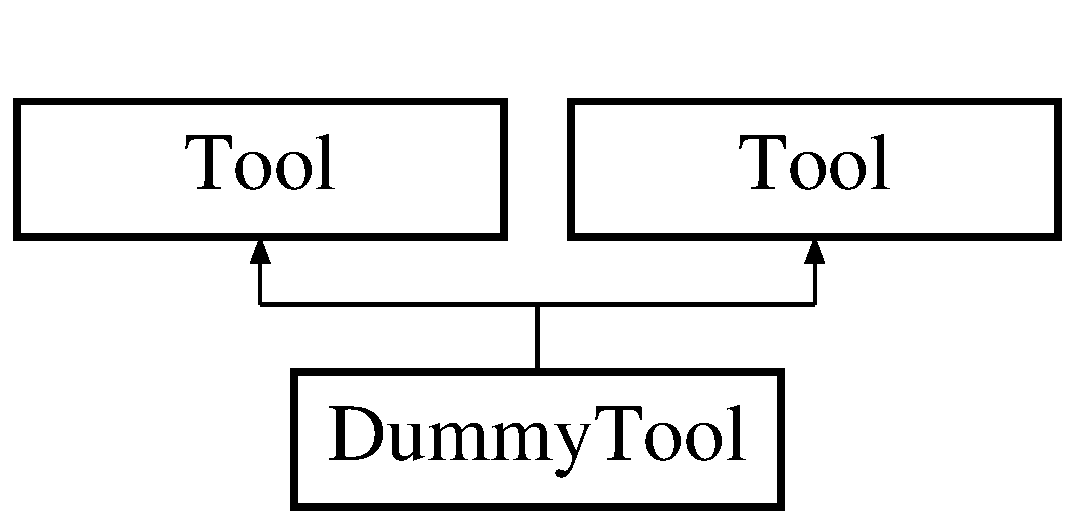
\includegraphics[height=2.000000cm]{classDummyTool}
\end{center}
\end{figure}
\subsection*{Public Member Functions}
\begin{DoxyCompactItemize}
\item 
\hypertarget{classDummyTool_a33914471b4de346168aa92b5febb6f9c}{\hyperlink{classDummyTool_a33914471b4de346168aa92b5febb6f9c}{Dummy\-Tool} ()}\label{classDummyTool_a33914471b4de346168aa92b5febb6f9c}

\begin{DoxyCompactList}\small\item\em Constructor. \end{DoxyCompactList}\item 
\hypertarget{classDummyTool_a0d9cd781681a06ee3cf0cd1e7bb770a8}{bool \hyperlink{classDummyTool_a0d9cd781681a06ee3cf0cd1e7bb770a8}{Initialise} (std\-::string configfile, \hyperlink{classDataModel}{Data\-Model} \&data)}\label{classDummyTool_a0d9cd781681a06ee3cf0cd1e7bb770a8}

\begin{DoxyCompactList}\small\item\em Assigns verbosity from config file and creates a log message. \end{DoxyCompactList}\item 
\hypertarget{classDummyTool_ac107b31f1785c1cc803e0e65be548047}{bool \hyperlink{classDummyTool_ac107b31f1785c1cc803e0e65be548047}{Execute} ()}\label{classDummyTool_ac107b31f1785c1cc803e0e65be548047}

\begin{DoxyCompactList}\small\item\em Creates a log message. \end{DoxyCompactList}\item 
\hypertarget{classDummyTool_aacb5d0b9906a27c2b4bba4aae9bc093a}{bool \hyperlink{classDummyTool_aacb5d0b9906a27c2b4bba4aae9bc093a}{Finalise} ()}\label{classDummyTool_aacb5d0b9906a27c2b4bba4aae9bc093a}

\begin{DoxyCompactList}\small\item\em Does nothing. \end{DoxyCompactList}\end{DoxyCompactItemize}
\subsection*{Additional Inherited Members}


\subsection{Detailed Description}
This is a simple dummy \hyperlink{classTool}{Tool} designed to show operation of a \hyperlink{classTool}{Tool}. It also provides a default \hyperlink{classTool}{Tool} for the Default \hyperlink{classToolChain}{Tool\-Chain}.

\begin{DoxyParagraph}{Author\-:}
B.\-Richards 
\end{DoxyParagraph}
\begin{DoxyParagraph}{Date\-:}
2019/05/28 10\-:44\-:00 
\end{DoxyParagraph}
Contact\-: \href{mailto:b.richards@qmul.ac.uk}{\tt b.\-richards@qmul.\-ac.\-uk} 

The documentation for this class was generated from the following files\-:\begin{DoxyCompactItemize}
\item 
User\-Tools/\-Dummy\-Tool/Dummy\-Tool.\-h\item 
User\-Tools/\-Dummy\-Tool/Dummy\-Tool.\-cpp\end{DoxyCompactItemize}

\hypertarget{classLogger}{\section{Logger Class Reference}
\label{classLogger}\index{Logger@{Logger}}
}


{\ttfamily \#include $<$Logger.\-h$>$}

Inheritance diagram for Logger\-:\begin{figure}[H]
\begin{center}
\leavevmode
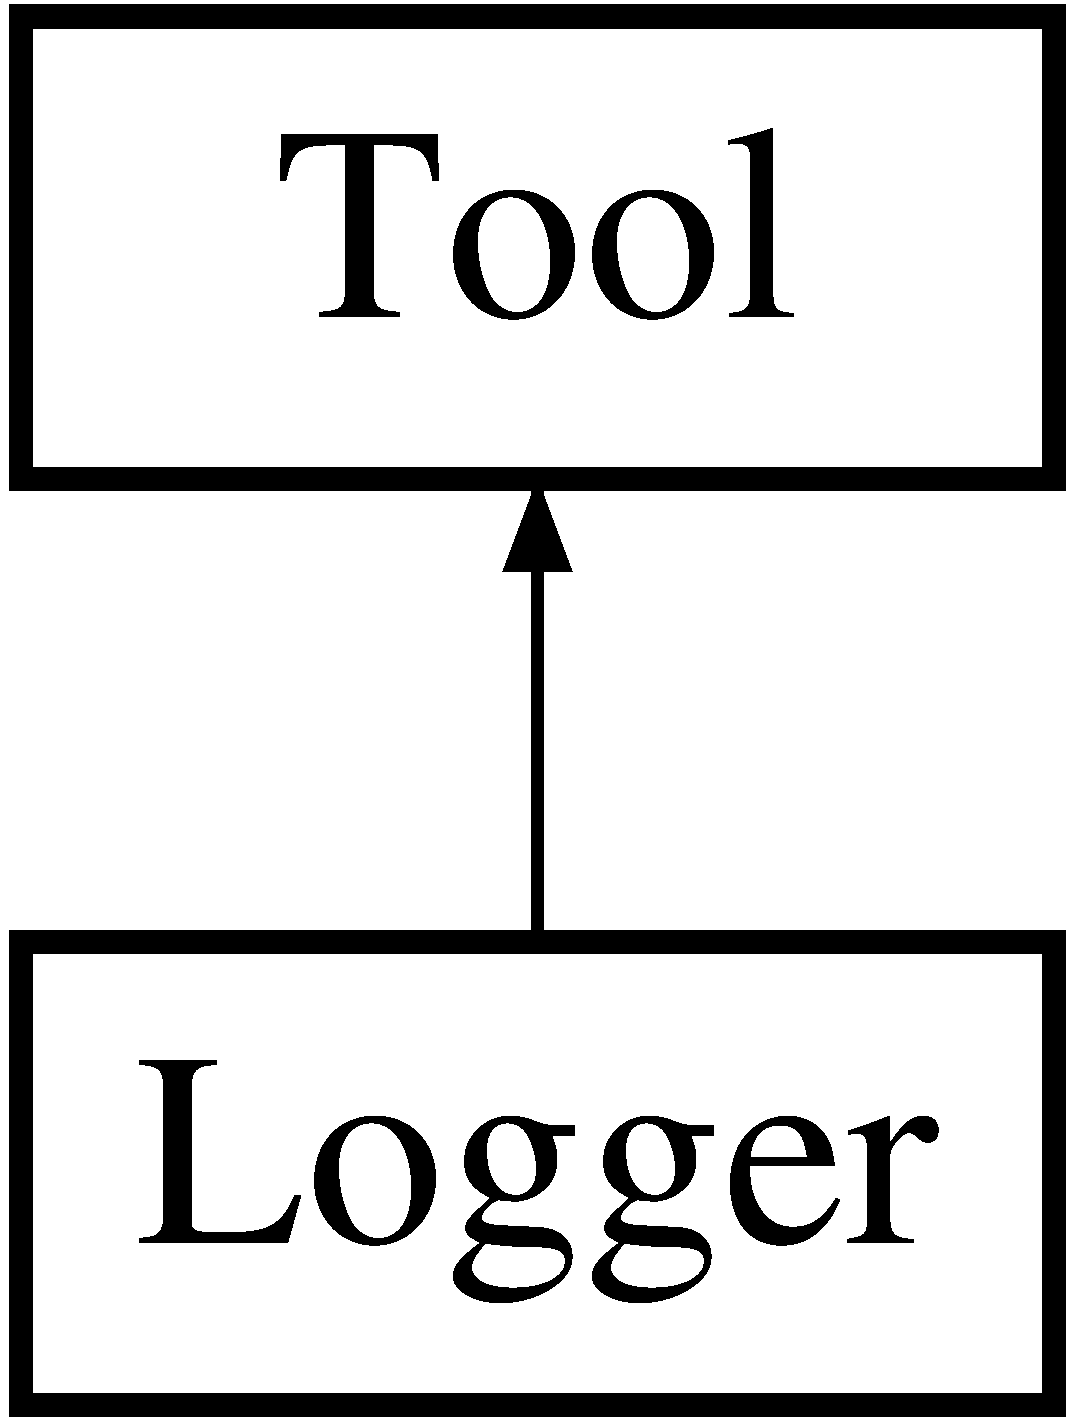
\includegraphics[height=2.000000cm]{classLogger}
\end{center}
\end{figure}
\subsection*{Public Member Functions}
\begin{DoxyCompactItemize}
\item 
\hypertarget{classLogger_abc41bfb031d896170c7675fa96a6b30c}{\hyperlink{classLogger_abc41bfb031d896170c7675fa96a6b30c}{Logger} ()}\label{classLogger_abc41bfb031d896170c7675fa96a6b30c}

\begin{DoxyCompactList}\small\item\em Construtor. \end{DoxyCompactList}\item 
\hypertarget{classLogger_a1b598f35f454e24f9e9abc9f18c3e98f}{bool \hyperlink{classLogger_a1b598f35f454e24f9e9abc9f18c3e98f}{Initialise} (std\-::string configfile, \hyperlink{classDataModel}{Data\-Model} \&data)}\label{classLogger_a1b598f35f454e24f9e9abc9f18c3e98f}

\begin{DoxyCompactList}\small\item\em Sets up a Z\-M\-Q\-\_\-\-P\-U\-L\-L socket which on the log part form the config file. \end{DoxyCompactList}\item 
\hypertarget{classLogger_a140ebede2975159a5abe7c59e56ec0ec}{bool \hyperlink{classLogger_a140ebede2975159a5abe7c59e56ec0ec}{Execute} ()}\label{classLogger_a140ebede2975159a5abe7c59e56ec0ec}

\begin{DoxyCompactList}\small\item\em Listens on socket for logging message printing them to screen when received. \end{DoxyCompactList}\item 
\hypertarget{classLogger_a2c70367a86d5999db21324ccb58f44ed}{bool \hyperlink{classLogger_a2c70367a86d5999db21324ccb58f44ed}{Finalise} ()}\label{classLogger_a2c70367a86d5999db21324ccb58f44ed}

\begin{DoxyCompactList}\small\item\em Closes socket and cleans up. \end{DoxyCompactList}\end{DoxyCompactItemize}
\subsection*{Additional Inherited Members}


\subsection{Detailed Description}
This is a demonstration tool that can receive \hyperlink{classLogging}{Logging} messages from Tool\-Chains

\begin{DoxyParagraph}{Author\-:}
B.\-Richards 
\end{DoxyParagraph}
\begin{DoxyParagraph}{Date\-:}
2019/05/28 10\-:44\-:00 
\end{DoxyParagraph}
Contact\-: \href{mailto:b.richards@qmul.ac.uk}{\tt b.\-richards@qmul.\-ac.\-uk} 

The documentation for this class was generated from the following files\-:\begin{DoxyCompactItemize}
\item 
User\-Tools/\-Logger/Logger.\-h\item 
User\-Tools/\-Logger/Logger.\-cpp\end{DoxyCompactItemize}

\hypertarget{classLogging}{\section{Logging Class Reference}
\label{classLogging}\index{Logging@{Logging}}
}


{\ttfamily \#include $<$Logging.\-h$>$}

Inheritance diagram for Logging\-:\begin{figure}[H]
\begin{center}
\leavevmode
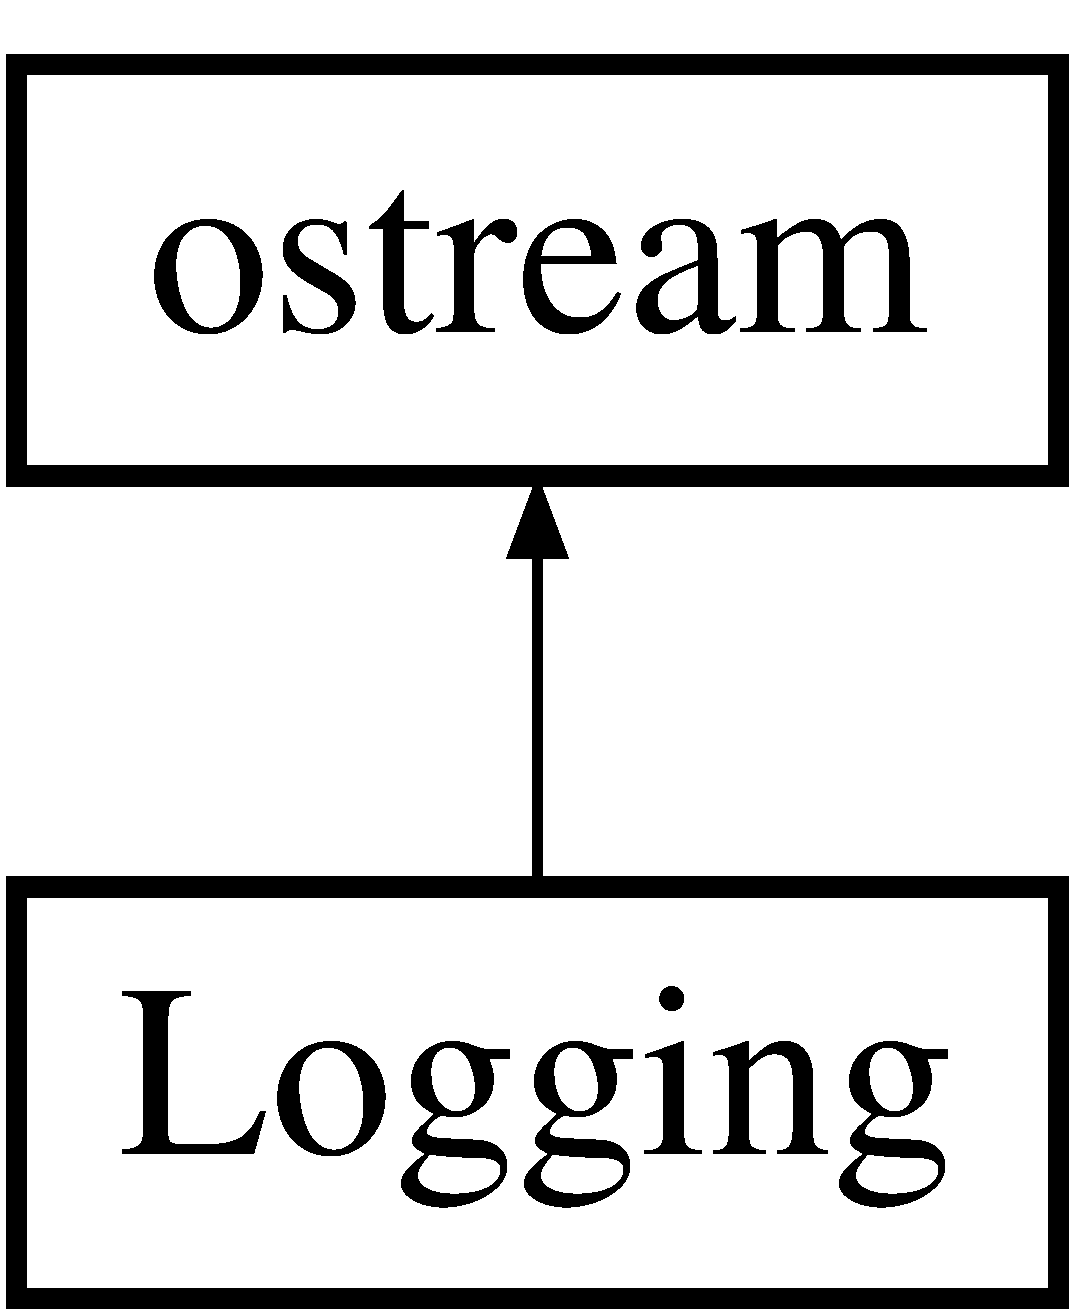
\includegraphics[height=2.000000cm]{classLogging}
\end{center}
\end{figure}
\subsection*{Public Member Functions}
\begin{DoxyCompactItemize}
\item 
\hyperlink{classLogging_ae7cc7299c697019f273b75cbfefff848}{Logging} (std\-::ostream \&str, zmq\-::context\-\_\-t $\ast$context, boost\-::uuids\-::uuid U\-U\-I\-D, std\-::string service, std\-::string mode, std\-::string localpath=\char`\"{}\char`\"{}, std\-::string logservice=\char`\"{}\char`\"{}, int logport=0)
\item 
{\footnotesize template$<$typename T $>$ }\\void \hyperlink{classLogging_af7839ee68729b066da269cc012b1fcc9}{Log} (T message, int messagelevel=1, int verbose=1)
\item 
bool \hyperlink{classLogging_a7a0c89c152ad81fb41a849ed9d81e429}{Change\-Out\-File} (std\-::string localpath)
\item 
\hyperlink{classLogging_ae7cc7299c697019f273b75cbfefff848}{Logging} (std\-::ostream \&str, zmq\-::context\-\_\-t $\ast$context, boost\-::uuids\-::uuid U\-U\-I\-D, std\-::string service, std\-::string mode, std\-::string localpath=\char`\"{}\char`\"{}, std\-::string logservice=\char`\"{}\char`\"{}, int logport=0)
\item 
{\footnotesize template$<$typename T $>$ }\\void \hyperlink{classLogging_af7839ee68729b066da269cc012b1fcc9}{Log} (T message, int messagelevel=1, int verbose=1)
\item 
bool \hyperlink{classLogging_a7a0c89c152ad81fb41a849ed9d81e429}{Change\-Out\-File} (std\-::string localpath)
\end{DoxyCompactItemize}
\subsection*{Public Attributes}
\begin{DoxyCompactItemize}
\item 
\hypertarget{classLogging_a9622376d4c126c163334149cabc98bcc}{My\-Stream\-Buf \hyperlink{classLogging_a9622376d4c126c163334149cabc98bcc}{buffer}}\label{classLogging_a9622376d4c126c163334149cabc98bcc}

\begin{DoxyCompactList}\small\item\em Stream buffer used to replace std\-::cout for redirection to coustom output. \end{DoxyCompactList}\end{DoxyCompactItemize}


\subsection{Detailed Description}
This class handels the logging, which can be directed to screen or file or over the via the \hyperlink{classToolChain}{Tool\-Chain} Config file

\begin{DoxyParagraph}{Author\-:}
B.\-Richards 
\end{DoxyParagraph}
\begin{DoxyParagraph}{Date\-:}
2019/05/27 18\-:34\-:00 
\end{DoxyParagraph}
Contact\-: \href{mailto:b.richards@qmul.ac.uk}{\tt b.\-richards@qmul.\-ac.\-uk} 

\subsection{Constructor \& Destructor Documentation}
\hypertarget{classLogging_ae7cc7299c697019f273b75cbfefff848}{\index{Logging@{Logging}!Logging@{Logging}}
\index{Logging@{Logging}!Logging@{Logging}}
\subsubsection[{Logging}]{\setlength{\rightskip}{0pt plus 5cm}Logging\-::\-Logging (
\begin{DoxyParamCaption}
\item[{std\-::ostream \&}]{str, }
\item[{zmq\-::context\-\_\-t $\ast$}]{context, }
\item[{boost\-::uuids\-::uuid}]{U\-U\-I\-D, }
\item[{std\-::string}]{service, }
\item[{std\-::string}]{mode, }
\item[{std\-::string}]{localpath = {\ttfamily \char`\"{}\char`\"{}}, }
\item[{std\-::string}]{logservice = {\ttfamily \char`\"{}\char`\"{}}, }
\item[{int}]{logport = {\ttfamily 0}}
\end{DoxyParamCaption}
)\hspace{0.3cm}{\ttfamily [inline]}}}\label{classLogging_ae7cc7299c697019f273b75cbfefff848}
Constructor for \hyperlink{classLogging}{Logging} class


\begin{DoxyParams}{Parameters}
{\em str} & \\
\hline
{\em context} & Pointer to Z\-M\-W context used for creating sockets \\
\hline
{\em U\-U\-I\-D} & \hyperlink{classToolChain}{Tool\-Chain} U\-U\-I\-D for unique labelling of log messages \\
\hline
{\em service} & \\
\hline
{\em mode} & \\
\hline
{\em localpath} & Local path for log output file \\
\hline
{\em logservice} & Remote service to connect to to send logs \\
\hline
{\em logport} & remothe port to send logging information to \\
\hline
\end{DoxyParams}
\hypertarget{classLogging_ae7cc7299c697019f273b75cbfefff848}{\index{Logging@{Logging}!Logging@{Logging}}
\index{Logging@{Logging}!Logging@{Logging}}
\subsubsection[{Logging}]{\setlength{\rightskip}{0pt plus 5cm}Logging\-::\-Logging (
\begin{DoxyParamCaption}
\item[{std\-::ostream \&}]{str, }
\item[{zmq\-::context\-\_\-t $\ast$}]{context, }
\item[{boost\-::uuids\-::uuid}]{U\-U\-I\-D, }
\item[{std\-::string}]{service, }
\item[{std\-::string}]{mode, }
\item[{std\-::string}]{localpath = {\ttfamily \char`\"{}\char`\"{}}, }
\item[{std\-::string}]{logservice = {\ttfamily \char`\"{}\char`\"{}}, }
\item[{int}]{logport = {\ttfamily 0}}
\end{DoxyParamCaption}
)\hspace{0.3cm}{\ttfamily [inline]}}}\label{classLogging_ae7cc7299c697019f273b75cbfefff848}
Constructor for \hyperlink{classLogging}{Logging} class


\begin{DoxyParams}{Parameters}
{\em str} & \\
\hline
{\em context} & Pointer to Z\-M\-W context used for creating sockets \\
\hline
{\em U\-U\-I\-D} & \hyperlink{classToolChain}{Tool\-Chain} U\-U\-I\-D for unique labelling of log messages \\
\hline
{\em service} & \\
\hline
{\em mode} & \\
\hline
{\em localpath} & Local path for log output file \\
\hline
{\em logservice} & Remote service to connect to to send logs \\
\hline
{\em logport} & remothe port to send logging information to \\
\hline
\end{DoxyParams}


\subsection{Member Function Documentation}
\hypertarget{classLogging_a7a0c89c152ad81fb41a849ed9d81e429}{\index{Logging@{Logging}!Change\-Out\-File@{Change\-Out\-File}}
\index{Change\-Out\-File@{Change\-Out\-File}!Logging@{Logging}}
\subsubsection[{Change\-Out\-File}]{\setlength{\rightskip}{0pt plus 5cm}bool Logging\-::\-Change\-Out\-File (
\begin{DoxyParamCaption}
\item[{std\-::string}]{localpath}
\end{DoxyParamCaption}
)\hspace{0.3cm}{\ttfamily [inline]}}}\label{classLogging_a7a0c89c152ad81fb41a849ed9d81e429}
Functionn to change the logs out file if set to a local path.


\begin{DoxyParams}{Parameters}
{\em localpath} & path to new log file. \\
\hline
\end{DoxyParams}
\begin{DoxyReturn}{Returns}
value is bool success of opening new logfile. 
\end{DoxyReturn}
\hypertarget{classLogging_a7a0c89c152ad81fb41a849ed9d81e429}{\index{Logging@{Logging}!Change\-Out\-File@{Change\-Out\-File}}
\index{Change\-Out\-File@{Change\-Out\-File}!Logging@{Logging}}
\subsubsection[{Change\-Out\-File}]{\setlength{\rightskip}{0pt plus 5cm}bool Logging\-::\-Change\-Out\-File (
\begin{DoxyParamCaption}
\item[{std\-::string}]{localpath}
\end{DoxyParamCaption}
)\hspace{0.3cm}{\ttfamily [inline]}}}\label{classLogging_a7a0c89c152ad81fb41a849ed9d81e429}
Functionn to change the logs out file if set to a local path.


\begin{DoxyParams}{Parameters}
{\em localpath} & path to new log file. \\
\hline
\end{DoxyParams}
\begin{DoxyReturn}{Returns}
value is bool success of opening new logfile. 
\end{DoxyReturn}
\hypertarget{classLogging_af7839ee68729b066da269cc012b1fcc9}{\index{Logging@{Logging}!Log@{Log}}
\index{Log@{Log}!Logging@{Logging}}
\subsubsection[{Log}]{\setlength{\rightskip}{0pt plus 5cm}template$<$typename T $>$ void Logging\-::\-Log (
\begin{DoxyParamCaption}
\item[{T}]{message, }
\item[{int}]{messagelevel = {\ttfamily 1}, }
\item[{int}]{verbose = {\ttfamily 1}}
\end{DoxyParamCaption}
)\hspace{0.3cm}{\ttfamily [inline]}}}\label{classLogging_af7839ee68729b066da269cc012b1fcc9}
Function to create a log messages.


\begin{DoxyParams}{Parameters}
{\em message} & templated log message text. \\
\hline
{\em messagelevel} & message verbosity level of the message being sent (e.\-g. if 'messagelevel$>$= verbose' Then message is sent). \\
\hline
{\em verbose} & verbosity level of the current \hyperlink{classTool}{Tool}. \\
\hline
\end{DoxyParams}
\hypertarget{classLogging_af7839ee68729b066da269cc012b1fcc9}{\index{Logging@{Logging}!Log@{Log}}
\index{Log@{Log}!Logging@{Logging}}
\subsubsection[{Log}]{\setlength{\rightskip}{0pt plus 5cm}template$<$typename T $>$ void Logging\-::\-Log (
\begin{DoxyParamCaption}
\item[{T}]{message, }
\item[{int}]{messagelevel = {\ttfamily 1}, }
\item[{int}]{verbose = {\ttfamily 1}}
\end{DoxyParamCaption}
)\hspace{0.3cm}{\ttfamily [inline]}}}\label{classLogging_af7839ee68729b066da269cc012b1fcc9}
Function to create a log messages.


\begin{DoxyParams}{Parameters}
{\em message} & templated log message text. \\
\hline
{\em messagelevel} & message verbosity level of the message being sent (e.\-g. if 'messagelevel$>$= verbose' Then message is sent). \\
\hline
{\em verbose} & verbosity level of the current \hyperlink{classTool}{Tool}. \\
\hline
\end{DoxyParams}


The documentation for this class was generated from the following files\-:\begin{DoxyCompactItemize}
\item 
include/Logging.\-h\item 
src/\-Logging/Logging.\-h\end{DoxyCompactItemize}

\hypertarget{structLogging__thread__args}{\section{Logging\-\_\-thread\-\_\-args Struct Reference}
\label{structLogging__thread__args}\index{Logging\-\_\-thread\-\_\-args@{Logging\-\_\-thread\-\_\-args}}
}


{\ttfamily \#include $<$Logging.\-h$>$}

\subsection*{Public Member Functions}
\begin{DoxyCompactItemize}
\item 
\hypertarget{structLogging__thread__args_a9496cec11539e17b104d3cbdf3174fdb}{\hyperlink{structLogging__thread__args_a9496cec11539e17b104d3cbdf3174fdb}{Logging\-\_\-thread\-\_\-args} (zmq\-::context\-\_\-t $\ast$incontext, boost\-::uuids\-::uuid in\-U\-U\-I\-D, std\-::string inlogservice, int inlogport)}\label{structLogging__thread__args_a9496cec11539e17b104d3cbdf3174fdb}

\begin{DoxyCompactList}\small\item\em Simple constructor to assign thread variables. \end{DoxyCompactList}\end{DoxyCompactItemize}
\subsection*{Public Attributes}
\begin{DoxyCompactItemize}
\item 
\hypertarget{structLogging__thread__args_addacf7a55861c13832a75b88d74c006c}{zmq\-::context\-\_\-t $\ast$ \hyperlink{structLogging__thread__args_addacf7a55861c13832a75b88d74c006c}{context}}\label{structLogging__thread__args_addacf7a55861c13832a75b88d74c006c}

\begin{DoxyCompactList}\small\item\em pointer to Z\-M\-Q context for socket creation \end{DoxyCompactList}\item 
\hypertarget{structLogging__thread__args_a3a7c5617b7fa5214c6da407a23266d57}{boost\-::uuids\-::uuid \hyperlink{structLogging__thread__args_a3a7c5617b7fa5214c6da407a23266d57}{U\-U\-I\-D}}\label{structLogging__thread__args_a3a7c5617b7fa5214c6da407a23266d57}

\begin{DoxyCompactList}\small\item\em \hyperlink{classToolChain}{Tool\-Chain} U\-U\-I\-D for unique labelling of log messages. \end{DoxyCompactList}\item 
\hypertarget{structLogging__thread__args_a5a8e255209f5c171a7fbd78f0e308087}{std\-::string \hyperlink{structLogging__thread__args_a5a8e255209f5c171a7fbd78f0e308087}{logservice}}\label{structLogging__thread__args_a5a8e255209f5c171a7fbd78f0e308087}

\begin{DoxyCompactList}\small\item\em Remote service name to connect to. \end{DoxyCompactList}\item 
\hypertarget{structLogging__thread__args_ad5ab1c21e226a694c7f813bcb3ef9002}{int \hyperlink{structLogging__thread__args_ad5ab1c21e226a694c7f813bcb3ef9002}{logport}}\label{structLogging__thread__args_ad5ab1c21e226a694c7f813bcb3ef9002}

\begin{DoxyCompactList}\small\item\em Port to connect to to send remote logging information. \end{DoxyCompactList}\end{DoxyCompactItemize}


\subsection{Detailed Description}
This struct holds the initalisation variables to be passed to the logging thread.

\begin{DoxyParagraph}{Author\-:}
B.\-Richards 
\end{DoxyParagraph}
\begin{DoxyParagraph}{Date\-:}
2019/05/27 18\-:34\-:00 
\end{DoxyParagraph}
Contact\-: \href{mailto:b.richards@qmul.ac.uk}{\tt b.\-richards@qmul.\-ac.\-uk} 

The documentation for this struct was generated from the following file\-:\begin{DoxyCompactItemize}
\item 
src/\-Logging/Logging.\-h\end{DoxyCompactItemize}

\hypertarget{classMyTool}{\section{My\-Tool Class Reference}
\label{classMyTool}\index{My\-Tool@{My\-Tool}}
}
Inheritance diagram for My\-Tool\-:\begin{figure}[H]
\begin{center}
\leavevmode
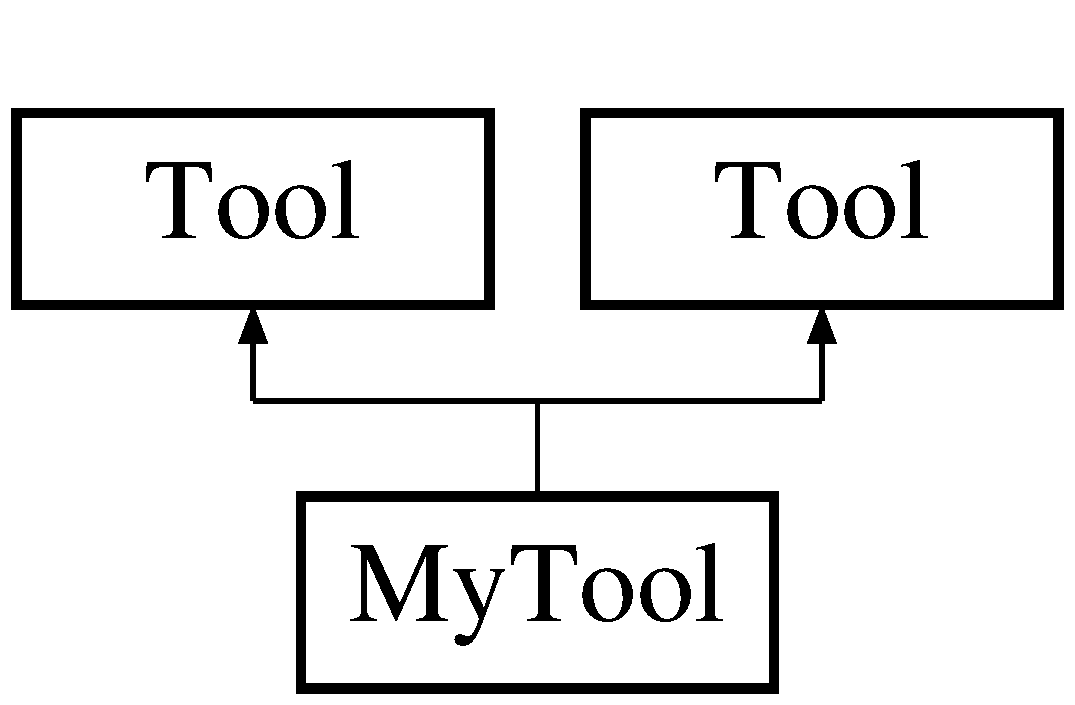
\includegraphics[height=2.000000cm]{classMyTool}
\end{center}
\end{figure}
\subsection*{Public Member Functions}
\begin{DoxyCompactItemize}
\item 
\hypertarget{classMyTool_a3bf60061195a18542c4cfb2916b9dad9}{bool {\bfseries Initialise} (std\-::string configfile, \hyperlink{classDataModel}{Data\-Model} \&data)}\label{classMyTool_a3bf60061195a18542c4cfb2916b9dad9}

\item 
\hypertarget{classMyTool_a0a58122023af90b9200d0e71e89cfb36}{bool {\bfseries Execute} ()}\label{classMyTool_a0a58122023af90b9200d0e71e89cfb36}

\item 
\hypertarget{classMyTool_a060ec6356451aa335d0de41093c9992f}{bool {\bfseries Finalise} ()}\label{classMyTool_a060ec6356451aa335d0de41093c9992f}

\end{DoxyCompactItemize}
\subsection*{Additional Inherited Members}


The documentation for this class was generated from the following file\-:\begin{DoxyCompactItemize}
\item 
include/My\-Tool.\-h\end{DoxyCompactItemize}

\hypertarget{classPointerWrapper}{\section{Pointer\-Wrapper$<$ T $>$ Class Template Reference}
\label{classPointerWrapper}\index{Pointer\-Wrapper$<$ T $>$@{Pointer\-Wrapper$<$ T $>$}}
}
Inheritance diagram for Pointer\-Wrapper$<$ T $>$\-:\begin{figure}[H]
\begin{center}
\leavevmode
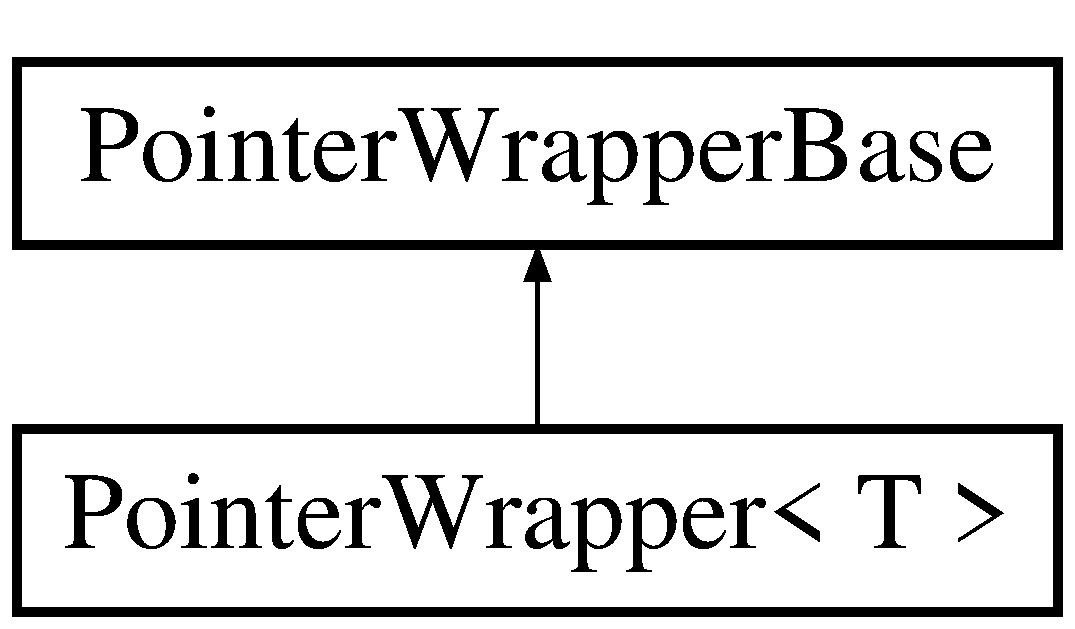
\includegraphics[height=2.000000cm]{classPointerWrapper}
\end{center}
\end{figure}
\subsection*{Public Member Functions}
\begin{DoxyCompactItemize}
\item 
\hypertarget{classPointerWrapper_aa645eb1963f91c9bddf5fd6ff578751b}{{\bfseries Pointer\-Wrapper} (T $\ast$inpointer)}\label{classPointerWrapper_aa645eb1963f91c9bddf5fd6ff578751b}

\end{DoxyCompactItemize}
\subsection*{Public Attributes}
\begin{DoxyCompactItemize}
\item 
\hypertarget{classPointerWrapper_a4866798d33eed0a9aeaa3bcda53c4a0d}{T $\ast$ {\bfseries pointer}}\label{classPointerWrapper_a4866798d33eed0a9aeaa3bcda53c4a0d}

\end{DoxyCompactItemize}


The documentation for this class was generated from the following file\-:\begin{DoxyCompactItemize}
\item 
include/Pointer\-Wrapper.\-h\end{DoxyCompactItemize}

\hypertarget{classPointerWrapperBase}{\section{Pointer\-Wrapper\-Base Class Reference}
\label{classPointerWrapperBase}\index{Pointer\-Wrapper\-Base@{Pointer\-Wrapper\-Base}}
}


{\ttfamily \#include $<$Pointer\-Wrapper.\-h$>$}

Inheritance diagram for Pointer\-Wrapper\-Base\-:\begin{figure}[H]
\begin{center}
\leavevmode
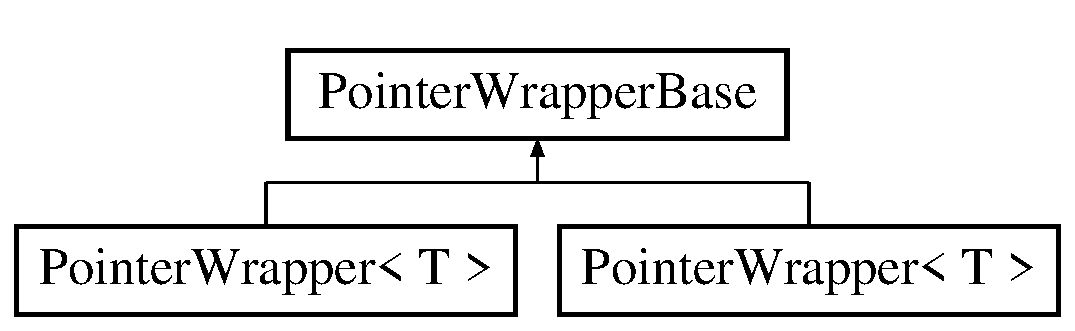
\includegraphics[height=2.000000cm]{classPointerWrapperBase}
\end{center}
\end{figure}
\subsection*{Public Member Functions}
\begin{DoxyCompactItemize}
\item 
\hypertarget{classPointerWrapperBase_ac9e248557a8aa248bcbbadc469c77f52}{\hyperlink{classPointerWrapperBase_ac9e248557a8aa248bcbbadc469c77f52}{Pointer\-Wrapper\-Base} ()}\label{classPointerWrapperBase_ac9e248557a8aa248bcbbadc469c77f52}

\begin{DoxyCompactList}\small\item\em Simple constructor. \end{DoxyCompactList}\item 
\hypertarget{classPointerWrapperBase_a842fb0af38187d71678971452c1e1094}{virtual \hyperlink{classPointerWrapperBase_a842fb0af38187d71678971452c1e1094}{$\sim$\-Pointer\-Wrapper\-Base} ()}\label{classPointerWrapperBase_a842fb0af38187d71678971452c1e1094}

\begin{DoxyCompactList}\small\item\em virtual destructor \end{DoxyCompactList}\end{DoxyCompactItemize}


\subsection{Detailed Description}
This class is used to wrap pointers stored in a \hyperlink{classBoostStore}{Boost\-Store}. It gives a generic abstract base class to store pointers under

\begin{DoxyParagraph}{Author\-:}
B.\-Richards 
\end{DoxyParagraph}
\begin{DoxyParagraph}{Date\-:}
2019/05/28 10\-:44\-:00 
\end{DoxyParagraph}
Contact\-: \href{mailto:b.richards@qmul.ac.uk}{\tt b.\-richards@qmul.\-ac.\-uk} 

The documentation for this class was generated from the following file\-:\begin{DoxyCompactItemize}
\item 
src/\-Store/Pointer\-Wrapper.\-h\end{DoxyCompactItemize}

\hypertarget{classSerialisableObject}{\section{Serialisable\-Object Class Reference}
\label{classSerialisableObject}\index{Serialisable\-Object@{Serialisable\-Object}}
}


{\ttfamily \#include $<$Serialisable\-Object.\-h$>$}

\subsection*{Public Member Functions}
\begin{DoxyCompactItemize}
\item 
\hypertarget{classSerialisableObject_a9055c98969917d4c652eefdc924b6b75}{virtual bool \hyperlink{classSerialisableObject_a9055c98969917d4c652eefdc924b6b75}{Print} ()=0}\label{classSerialisableObject_a9055c98969917d4c652eefdc924b6b75}

\begin{DoxyCompactList}\small\item\em Simple virtual Pritn function to ensure inhereted classes have one. \end{DoxyCompactList}\end{DoxyCompactItemize}
\subsection*{Public Attributes}
\begin{DoxyCompactItemize}
\item 
bool \hyperlink{classSerialisableObject_a4635f9e80623df463bcca2c88b10fc67}{serialise}
\begin{DoxyCompactList}\small\item\em Destructor. \end{DoxyCompactList}\end{DoxyCompactItemize}
\subsection*{Protected Member Functions}
\begin{DoxyCompactItemize}
\item 
{\footnotesize template$<$class Archive $>$ }\\void \hyperlink{classSerialisableObject_a7c9ec7bf87b5921957768f4467c6143a}{serialize} (Archive \&ar, const unsigned int \hyperlink{classSerialisableObject_ade0071c238a09193b37a2750d2b50b18}{version})
\end{DoxyCompactItemize}
\subsection*{Protected Attributes}
\begin{DoxyCompactItemize}
\item 
\hypertarget{classSerialisableObject_a893f965e41ad7f09b4066cb07fecef8e}{std\-::string \hyperlink{classSerialisableObject_a893f965e41ad7f09b4066cb07fecef8e}{type}}\label{classSerialisableObject_a893f965e41ad7f09b4066cb07fecef8e}

\begin{DoxyCompactList}\small\item\em String to store type of \hyperlink{classTool}{Tool}. \end{DoxyCompactList}\item 
\hypertarget{classSerialisableObject_ade0071c238a09193b37a2750d2b50b18}{std\-::string \hyperlink{classSerialisableObject_ade0071c238a09193b37a2750d2b50b18}{version}}\label{classSerialisableObject_ade0071c238a09193b37a2750d2b50b18}

\begin{DoxyCompactList}\small\item\em String to store version of \hyperlink{classTool}{Tool}. \end{DoxyCompactList}\end{DoxyCompactItemize}
\subsection*{Friends}
\begin{DoxyCompactItemize}
\item 
\hypertarget{classSerialisableObject_ac98d07dd8f7b70e16ccb9a01abf56b9c}{class {\bfseries boost\-::serialization\-::access}}\label{classSerialisableObject_ac98d07dd8f7b70e16ccb9a01abf56b9c}

\end{DoxyCompactItemize}


\subsection{Detailed Description}
An abstract base class for sustom calsses to inherit from to ensure version and type information are present, as well as a Print function and some form of sereialisation.

\begin{DoxyParagraph}{Author\-:}
B.\-Richards 
\end{DoxyParagraph}
\begin{DoxyParagraph}{Date\-:}
2019/05/28 10\-:44\-:00 
\end{DoxyParagraph}
Contact\-: \href{mailto:b.richards@qmul.ac.uk}{\tt b.\-richards@qmul.\-ac.\-uk} 

\subsection{Member Function Documentation}
\hypertarget{classSerialisableObject_a7c9ec7bf87b5921957768f4467c6143a}{\index{Serialisable\-Object@{Serialisable\-Object}!serialize@{serialize}}
\index{serialize@{serialize}!SerialisableObject@{Serialisable\-Object}}
\subsubsection[{serialize}]{\setlength{\rightskip}{0pt plus 5cm}template$<$class Archive $>$ void Serialisable\-Object\-::serialize (
\begin{DoxyParamCaption}
\item[{Archive \&}]{ar, }
\item[{const unsigned int}]{version}
\end{DoxyParamCaption}
)\hspace{0.3cm}{\ttfamily [inline]}, {\ttfamily [protected]}}}\label{classSerialisableObject_a7c9ec7bf87b5921957768f4467c6143a}
Simple Boost serialise method to serialise the membervariables of a custom class. This shuld be expanded to include the custom classes variables 
\begin{DoxyParams}{Parameters}
{\em ar} & Boost archive. \\
\hline
{\em version} & of the archive. \\
\hline
\end{DoxyParams}


\subsection{Member Data Documentation}
\hypertarget{classSerialisableObject_a4635f9e80623df463bcca2c88b10fc67}{\index{Serialisable\-Object@{Serialisable\-Object}!serialise@{serialise}}
\index{serialise@{serialise}!SerialisableObject@{Serialisable\-Object}}
\subsubsection[{serialise}]{\setlength{\rightskip}{0pt plus 5cm}bool Serialisable\-Object\-::serialise}}\label{classSerialisableObject_a4635f9e80623df463bcca2c88b10fc67}


Destructor. 

Denotes if the calss should be serialised or not when added to a \hyperlink{classBoostStore}{Boost\-Store}. 

The documentation for this class was generated from the following file\-:\begin{DoxyCompactItemize}
\item 
src/\-Store/Serialisable\-Object.\-h\end{DoxyCompactItemize}

\hypertarget{classServiceAdd}{\section{Service\-Add Class Reference}
\label{classServiceAdd}\index{Service\-Add@{Service\-Add}}
}


{\ttfamily \#include $<$Service\-Add.\-h$>$}

Inheritance diagram for Service\-Add\-:\begin{figure}[H]
\begin{center}
\leavevmode
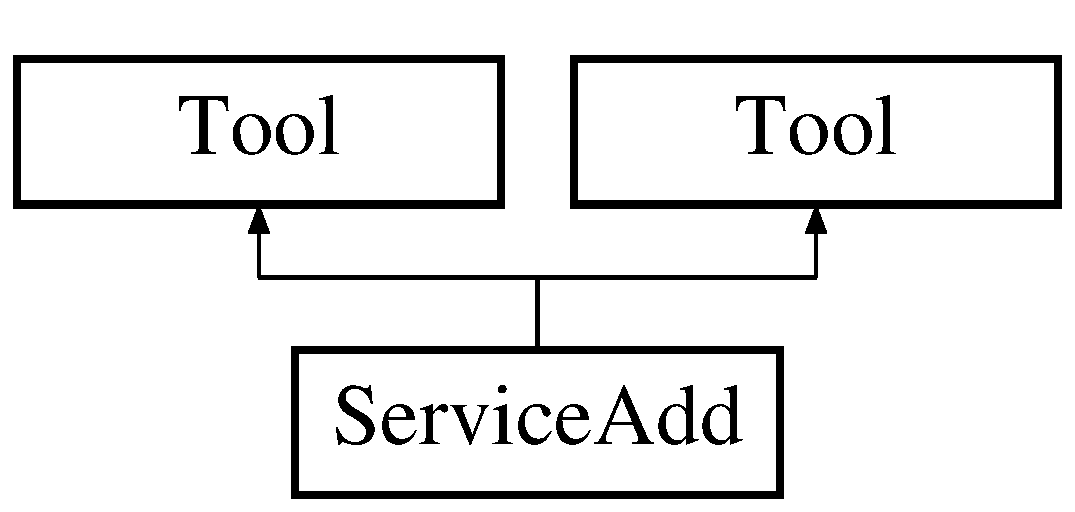
\includegraphics[height=2.000000cm]{classServiceAdd}
\end{center}
\end{figure}
\subsection*{Public Member Functions}
\begin{DoxyCompactItemize}
\item 
\hypertarget{classServiceAdd_a0148b0e038f4b0dd6f12c87cdf233f69}{\hyperlink{classServiceAdd_a0148b0e038f4b0dd6f12c87cdf233f69}{Service\-Add} ()}\label{classServiceAdd_a0148b0e038f4b0dd6f12c87cdf233f69}

\begin{DoxyCompactList}\small\item\em Constrcutor. \end{DoxyCompactList}\item 
\hypertarget{classServiceAdd_a047e44c3d209591703b0bdec1b1b51cd}{bool \hyperlink{classServiceAdd_a047e44c3d209591703b0bdec1b1b51cd}{Initialise} (std\-::string configfile, \hyperlink{classDataModel}{Data\-Model} \&data)}\label{classServiceAdd_a047e44c3d209591703b0bdec1b1b51cd}

\begin{DoxyCompactList}\small\item\em Opens socket to service discoverypublisher and adds a service and assosiated port to broadcast. \end{DoxyCompactList}\item 
\hypertarget{classServiceAdd_a4908df063074b02e73e589d9f07998ac}{bool \hyperlink{classServiceAdd_a4908df063074b02e73e589d9f07998ac}{Execute} ()}\label{classServiceAdd_a4908df063074b02e73e589d9f07998ac}

\begin{DoxyCompactList}\small\item\em Does nothing. \end{DoxyCompactList}\item 
\hypertarget{classServiceAdd_a2e4d3854bcd490935e6e9d39597c7204}{bool \hyperlink{classServiceAdd_a2e4d3854bcd490935e6e9d39597c7204}{Finalise} ()}\label{classServiceAdd_a2e4d3854bcd490935e6e9d39597c7204}

\begin{DoxyCompactList}\small\item\em Opens new connection to service discovery publish thread and removes service from service list. \end{DoxyCompactList}\end{DoxyCompactItemize}
\subsection*{Additional Inherited Members}


\subsection{Detailed Description}
This Tools demonstraits how to add services and publicise connections for them in the Tool\-Cahins multicast beacons.

\begin{DoxyParagraph}{Author\-:}
B.\-Richards 
\end{DoxyParagraph}
\begin{DoxyParagraph}{Date\-:}
2019/05/28 10\-:44\-:00 
\end{DoxyParagraph}
Contact\-: \href{mailto:b.richards@qmul.ac.uk}{\tt b.\-richards@qmul.\-ac.\-uk} 

The documentation for this class was generated from the following files\-:\begin{DoxyCompactItemize}
\item 
User\-Tools/\-Service\-Add/Service\-Add.\-h\item 
User\-Tools/\-Service\-Add/Service\-Add.\-cpp\end{DoxyCompactItemize}

\hypertarget{classServiceDiscovery}{\section{Service\-Discovery Class Reference}
\label{classServiceDiscovery}\index{Service\-Discovery@{Service\-Discovery}}
}
\subsection*{Public Member Functions}
\begin{DoxyCompactItemize}
\item 
\hypertarget{classServiceDiscovery_ab69c2cacaf5a388fac88e57f3361b576}{{\bfseries Service\-Discovery} (bool Send, bool Receive, int remoteport, std\-::string address, int multicastport, zmq\-::context\-\_\-t $\ast$incontext, boost\-::uuids\-::uuid U\-U\-I\-D, std\-::string service, int pubsec=5, int kicksec=60)}\label{classServiceDiscovery_ab69c2cacaf5a388fac88e57f3361b576}

\item 
\hypertarget{classServiceDiscovery_a3dbd15f19345b0c9746731308e26b034}{{\bfseries Service\-Discovery} (std\-::string address, int multicastport, zmq\-::context\-\_\-t $\ast$incontext, int kicksec=60)}\label{classServiceDiscovery_a3dbd15f19345b0c9746731308e26b034}

\end{DoxyCompactItemize}


The documentation for this class was generated from the following files\-:\begin{DoxyCompactItemize}
\item 
src/\-Service\-Discovery/Service\-Discovery.\-h\item 
src/\-Service\-Discovery/Service\-Discovery.\-cpp\end{DoxyCompactItemize}

\hypertarget{classStore}{\section{Store Class Reference}
\label{classStore}\index{Store@{Store}}
}
\subsection*{Public Member Functions}
\begin{DoxyCompactItemize}
\item 
\hypertarget{classStore_af5e0db5a37234365c4deb5bedd76693c}{void {\bfseries Initialise} (std\-::string filename)}\label{classStore_af5e0db5a37234365c4deb5bedd76693c}

\item 
\hypertarget{classStore_adb84e3fb286cae07f64e8186b7ab04e1}{void {\bfseries Json\-Parser} (std\-::string input)}\label{classStore_adb84e3fb286cae07f64e8186b7ab04e1}

\item 
\hypertarget{classStore_a9d2f000bd849a9f5de71c3ba62dca340}{void {\bfseries Print} ()}\label{classStore_a9d2f000bd849a9f5de71c3ba62dca340}

\item 
\hypertarget{classStore_a7fce0f8f3ec7978c5e7cd3d7053f899b}{void {\bfseries Delete} ()}\label{classStore_a7fce0f8f3ec7978c5e7cd3d7053f899b}

\item 
\hypertarget{classStore_abdc0134daa34b808328070f5d6b295f3}{{\footnotesize template$<$typename T $>$ }\\bool {\bfseries Get} (std\-::string name, T \&out)}\label{classStore_abdc0134daa34b808328070f5d6b295f3}

\item 
\hypertarget{classStore_af586739813ce18da6f5e3561d134a814}{{\footnotesize template$<$typename T $>$ }\\void {\bfseries Set} (std\-::string name, T in)}\label{classStore_af586739813ce18da6f5e3561d134a814}

\item 
\hypertarget{classStore_a790ca02bc7d11648edf0c8d5df3751fe}{std\-::string $\ast$ {\bfseries operator\mbox{[}$\,$\mbox{]}} (std\-::string key)}\label{classStore_a790ca02bc7d11648edf0c8d5df3751fe}

\item 
\hypertarget{classStore_abe9b65d1308c43dc4158b00d6aed7385}{{\footnotesize template$<$typename T $>$ }\\void {\bfseries operator$>$$>$} (T \&obj)}\label{classStore_abe9b65d1308c43dc4158b00d6aed7385}

\end{DoxyCompactItemize}
\subsection*{Friends}
\begin{DoxyCompactItemize}
\item 
\hypertarget{classStore_ac98d07dd8f7b70e16ccb9a01abf56b9c}{class {\bfseries boost\-::serialization\-::access}}\label{classStore_ac98d07dd8f7b70e16ccb9a01abf56b9c}

\end{DoxyCompactItemize}


The documentation for this class was generated from the following file\-:\begin{DoxyCompactItemize}
\item 
include/Store.\-h\end{DoxyCompactItemize}

\hypertarget{structthread__args}{\section{thread\-\_\-args Struct Reference}
\label{structthread__args}\index{thread\-\_\-args@{thread\-\_\-args}}
}
\subsection*{Public Member Functions}
\begin{DoxyCompactItemize}
\item 
\hypertarget{structthread__args_a6b3383444ec19a7bd2969229e1b87d2f}{{\bfseries thread\-\_\-args} (boost\-::uuids\-::uuid in\-U\-U\-I\-D, zmq\-::context\-\_\-t $\ast$incontext, std\-::string inmulticastaddress, int inmulticastport, std\-::string inservice, int inremoteport, int inpubsec=5, int inkicksec=5)}\label{structthread__args_a6b3383444ec19a7bd2969229e1b87d2f}

\end{DoxyCompactItemize}
\subsection*{Public Attributes}
\begin{DoxyCompactItemize}
\item 
\hypertarget{structthread__args_a707586ba05cc2c8be29cf22769b67634}{boost\-::uuids\-::uuid {\bfseries U\-U\-I\-D}}\label{structthread__args_a707586ba05cc2c8be29cf22769b67634}

\item 
\hypertarget{structthread__args_a217d01ac4eb4fd9c9ed1ebe4d02ca330}{zmq\-::context\-\_\-t $\ast$ {\bfseries context}}\label{structthread__args_a217d01ac4eb4fd9c9ed1ebe4d02ca330}

\item 
\hypertarget{structthread__args_a15f6bcc7a120e51d1074bb8703322ed5}{std\-::string {\bfseries multicastaddress}}\label{structthread__args_a15f6bcc7a120e51d1074bb8703322ed5}

\item 
\hypertarget{structthread__args_aa6059ab0eeca3f487491f2542bb5120b}{int {\bfseries multicastport}}\label{structthread__args_aa6059ab0eeca3f487491f2542bb5120b}

\item 
\hypertarget{structthread__args_a92798a7f2094db41f45ecbef0c067ca9}{std\-::string {\bfseries service}}\label{structthread__args_a92798a7f2094db41f45ecbef0c067ca9}

\item 
\hypertarget{structthread__args_a371407c82f7f64e3d9df634e59369565}{int {\bfseries remoteport}}\label{structthread__args_a371407c82f7f64e3d9df634e59369565}

\item 
\hypertarget{structthread__args_aba650f345201e8aece9071377945cf0e}{int {\bfseries pubsec}}\label{structthread__args_aba650f345201e8aece9071377945cf0e}

\item 
\hypertarget{structthread__args_a9b75103528b3a6fcc3dfc133cd1b1e8e}{int {\bfseries kicksec}}\label{structthread__args_a9b75103528b3a6fcc3dfc133cd1b1e8e}

\end{DoxyCompactItemize}


The documentation for this struct was generated from the following file\-:\begin{DoxyCompactItemize}
\item 
include/Service\-Discovery.\-h\end{DoxyCompactItemize}

\hypertarget{classTool}{\section{Tool Class Reference}
\label{classTool}\index{Tool@{Tool}}
}


{\ttfamily \#include $<$Tool.\-h$>$}

Inheritance diagram for Tool\-:\begin{figure}[H]
\begin{center}
\leavevmode
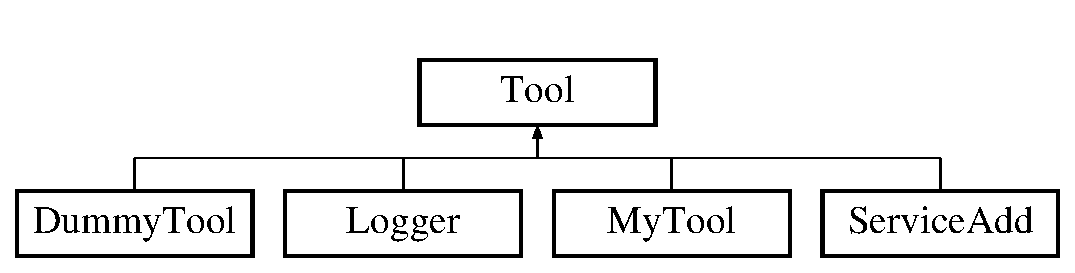
\includegraphics[height=2.000000cm]{classTool}
\end{center}
\end{figure}
\subsection*{Public Member Functions}
\begin{DoxyCompactItemize}
\item 
virtual bool \hyperlink{classTool_a4b04a99172dfe09dc97927d1feaff0ce}{Initialise} (std\-::string configfile, \hyperlink{classDataModel}{Data\-Model} \&data)=0
\begin{DoxyCompactList}\small\item\em virtual Initialise function that reads in the assigned config file and optain Data\-Moodel reference \end{DoxyCompactList}\item 
\hypertarget{classTool_a6a71469fa4efffd6fb71afbd4941e49d}{virtual bool \hyperlink{classTool_a6a71469fa4efffd6fb71afbd4941e49d}{Execute} ()=0}\label{classTool_a6a71469fa4efffd6fb71afbd4941e49d}

\begin{DoxyCompactList}\small\item\em Virtual Execute function. \end{DoxyCompactList}\item 
\hypertarget{classTool_a1f9a82fe5cc9afd63fc8eb3aaf5d80ca}{virtual bool \hyperlink{classTool_a1f9a82fe5cc9afd63fc8eb3aaf5d80ca}{Finalise} ()=0}\label{classTool_a1f9a82fe5cc9afd63fc8eb3aaf5d80ca}

\begin{DoxyCompactList}\small\item\em Virtual Finalise function. \end{DoxyCompactList}\end{DoxyCompactItemize}
\subsection*{Protected Member Functions}
\begin{DoxyCompactItemize}
\item 
{\footnotesize template$<$typename T $>$ }\\void \hyperlink{classTool_a46f7e599888302feefcf25e4f6cb4f9e}{Log} (T message, int messagelevel=1, int verbosity=1)
\begin{DoxyCompactList}\small\item\em \hyperlink{classLogging}{Logging} fuction for printouts. \end{DoxyCompactList}\end{DoxyCompactItemize}
\subsection*{Protected Attributes}
\begin{DoxyCompactItemize}
\item 
\hyperlink{classStore}{Store} \hyperlink{classTool_a208aed50c1c50212d2927b372c38763f}{m\-\_\-variables}
\begin{DoxyCompactList}\small\item\em virtual destructor. \end{DoxyCompactList}\item 
\hypertarget{classTool_a98d3ffa12f1de908da9030c8718ce3f5}{\hyperlink{classDataModel}{Data\-Model} $\ast$ \hyperlink{classTool_a98d3ffa12f1de908da9030c8718ce3f5}{m\-\_\-data}}\label{classTool_a98d3ffa12f1de908da9030c8718ce3f5}

\begin{DoxyCompactList}\small\item\em Pointer to transiant \hyperlink{classDataModel}{Data\-Model} class. \end{DoxyCompactList}\end{DoxyCompactItemize}


\subsection{Detailed Description}
Abstract base class for Tools to inherit from. This allows a polymphic interface for the factor to use.

\begin{DoxyParagraph}{Author\-:}
B.\-Richards 
\end{DoxyParagraph}
\begin{DoxyParagraph}{Date\-:}
2019/05/28 10\-:44\-:00 
\end{DoxyParagraph}
Contact\-: \href{mailto:b.richards@qmul.ac.uk}{\tt b.\-richards@qmul.\-ac.\-uk} 

\subsection{Member Function Documentation}
\hypertarget{classTool_a4b04a99172dfe09dc97927d1feaff0ce}{\index{Tool@{Tool}!Initialise@{Initialise}}
\index{Initialise@{Initialise}!Tool@{Tool}}
\subsubsection[{Initialise}]{\setlength{\rightskip}{0pt plus 5cm}virtual bool Tool\-::\-Initialise (
\begin{DoxyParamCaption}
\item[{std\-::string}]{configfile, }
\item[{{\bf Data\-Model} \&}]{data}
\end{DoxyParamCaption}
)\hspace{0.3cm}{\ttfamily [pure virtual]}}}\label{classTool_a4b04a99172dfe09dc97927d1feaff0ce}


virtual Initialise function that reads in the assigned config file and optain Data\-Moodel reference 


\begin{DoxyParams}{Parameters}
{\em configfile} & Path and name of config file to read in. \\
\hline
{\em data} & Reference to \hyperlink{classDataModel}{Data\-Model}. \\
\hline
\end{DoxyParams}


Implemented in \hyperlink{classServiceAdd_a047e44c3d209591703b0bdec1b1b51cd}{Service\-Add}, \hyperlink{classMyTool_a3bf60061195a18542c4cfb2916b9dad9}{My\-Tool}, \hyperlink{classDummyTool_a0d9cd781681a06ee3cf0cd1e7bb770a8}{Dummy\-Tool}, and \hyperlink{classLogger_a1b598f35f454e24f9e9abc9f18c3e98f}{Logger}.

\hypertarget{classTool_a46f7e599888302feefcf25e4f6cb4f9e}{\index{Tool@{Tool}!Log@{Log}}
\index{Log@{Log}!Tool@{Tool}}
\subsubsection[{Log}]{\setlength{\rightskip}{0pt plus 5cm}template$<$typename T $>$ void Tool\-::\-Log (
\begin{DoxyParamCaption}
\item[{T}]{message, }
\item[{int}]{messagelevel = {\ttfamily 1}, }
\item[{int}]{verbosity = {\ttfamily 1}}
\end{DoxyParamCaption}
)\hspace{0.3cm}{\ttfamily [inline]}, {\ttfamily [protected]}}}\label{classTool_a46f7e599888302feefcf25e4f6cb4f9e}


\hyperlink{classLogging}{Logging} fuction for printouts. 


\begin{DoxyParams}{Parameters}
{\em message} & Templated message string. \\
\hline
{\em messagelevel} & The verbosity level at which to show the message. \\
\hline
{\em verbosity} & The current verbosity level. \\
\hline
\end{DoxyParams}


\subsection{Member Data Documentation}
\hypertarget{classTool_a208aed50c1c50212d2927b372c38763f}{\index{Tool@{Tool}!m\-\_\-variables@{m\-\_\-variables}}
\index{m\-\_\-variables@{m\-\_\-variables}!Tool@{Tool}}
\subsubsection[{m\-\_\-variables}]{\setlength{\rightskip}{0pt plus 5cm}{\bf Store} Tool\-::m\-\_\-variables\hspace{0.3cm}{\ttfamily [protected]}}}\label{classTool_a208aed50c1c50212d2927b372c38763f}


virtual destructor. 

\hyperlink{classStore}{Store} used to store configuration varaibles 

The documentation for this class was generated from the following file\-:\begin{DoxyCompactItemize}
\item 
src/\-Tool/Tool.\-h\end{DoxyCompactItemize}

\hypertarget{classToolChain}{\section{Tool\-Chain Class Reference}
\label{classToolChain}\index{Tool\-Chain@{Tool\-Chain}}
}
\subsection*{Public Member Functions}
\begin{DoxyCompactItemize}
\item 
\hypertarget{classToolChain_a75af494cf7d613290c48fcbcdb700482}{{\bfseries Tool\-Chain} (std\-::string configfile)}\label{classToolChain_a75af494cf7d613290c48fcbcdb700482}

\item 
\hypertarget{classToolChain_a82c1596d9d6e233492e29ac83e2f8952}{{\bfseries Tool\-Chain} (int verbose=1, int errorlevel=0, std\-::string service=\char`\"{}test\char`\"{}, std\-::string logmode=\char`\"{}Interactive\char`\"{}, std\-::string log\-\_\-local\-\_\-path=\char`\"{}./log\char`\"{}, std\-::string log\-\_\-service=\char`\"{}\char`\"{}, int log\-\_\-port=0, int pub\-\_\-sec=5, int kick\-\_\-sec=60, unsigned int I\-O\-\_\-\-Threads=1)}\label{classToolChain_a82c1596d9d6e233492e29ac83e2f8952}

\item 
\hypertarget{classToolChain_a4da0c02154a0597704e58836d6607e61}{void {\bfseries Add} (std\-::string name, \hyperlink{classTool}{Tool} $\ast$tool, std\-::string configfile=\char`\"{}\char`\"{})}\label{classToolChain_a4da0c02154a0597704e58836d6607e61}

\item 
\hypertarget{classToolChain_a341f343926341b82a29c586a7b9683af}{int {\bfseries Initialise} ()}\label{classToolChain_a341f343926341b82a29c586a7b9683af}

\item 
\hypertarget{classToolChain_a303e299293fd4d3a5e91865e04898e52}{int {\bfseries Execute} (int repeates=1)}\label{classToolChain_a303e299293fd4d3a5e91865e04898e52}

\item 
\hypertarget{classToolChain_a3828756135773fb9ca4b361a47296dd9}{int {\bfseries Finalise} ()}\label{classToolChain_a3828756135773fb9ca4b361a47296dd9}

\item 
\hypertarget{classToolChain_a9bb47b83b6b85c3b0fab75af0cda19bf}{void {\bfseries Interactive} ()}\label{classToolChain_a9bb47b83b6b85c3b0fab75af0cda19bf}

\item 
\hypertarget{classToolChain_aacc213c07f81ee202dce14856a076df3}{void {\bfseries Remote} (int portnum, std\-::string S\-D\-\_\-address=\char`\"{}239.\-192.\-1.\-1\char`\"{}, int S\-D\-\_\-port=5000)}\label{classToolChain_aacc213c07f81ee202dce14856a076df3}

\end{DoxyCompactItemize}
\subsection*{Public Attributes}
\begin{DoxyCompactItemize}
\item 
\hypertarget{classToolChain_a92c81316d0c0b16ee9e4a084dd976f83}{\hyperlink{classDataModel}{Data\-Model} {\bfseries m\-\_\-data}}\label{classToolChain_a92c81316d0c0b16ee9e4a084dd976f83}

\end{DoxyCompactItemize}


The documentation for this class was generated from the following file\-:\begin{DoxyCompactItemize}
\item 
include/Tool\-Chain.\-h\end{DoxyCompactItemize}

\hypertarget{structToolChainargs}{\section{Tool\-Chainargs Struct Reference}
\label{structToolChainargs}\index{Tool\-Chainargs@{Tool\-Chainargs}}
}


{\ttfamily \#include $<$Tool\-Chain.\-h$>$}

\subsection*{Public Attributes}
\begin{DoxyCompactItemize}
\item 
\hypertarget{structToolChainargs_a288a3015acf712919f128c216eecadad}{zmq\-::context\-\_\-t $\ast$ \hyperlink{structToolChainargs_a288a3015acf712919f128c216eecadad}{context}}\label{structToolChainargs_a288a3015acf712919f128c216eecadad}

\begin{DoxyCompactList}\small\item\em Z\-M\-Q context used for creating sockets. \end{DoxyCompactList}\item 
\hypertarget{structToolChainargs_a3551269b039d543b844a2d0d924ce96b}{bool $\ast$ \hyperlink{structToolChainargs_a3551269b039d543b844a2d0d924ce96b}{msgflag}}\label{structToolChainargs_a3551269b039d543b844a2d0d924ce96b}

\begin{DoxyCompactList}\small\item\em Message flag used to indiacte if a new interactive command has been submitted to the interactive thread and needs execution on the main thread. \end{DoxyCompactList}\end{DoxyCompactItemize}


\subsection{Detailed Description}
Simple struct to pass thread initalisation variables to Interactive \hyperlink{classToolChain}{Tool\-Chain} thread

\begin{DoxyParagraph}{Author\-:}
B.\-Richards 
\end{DoxyParagraph}
\begin{DoxyParagraph}{Date\-:}
2019/05/28 10\-:44\-:00 
\end{DoxyParagraph}
Contact\-: \href{mailto:b.richards@qmul.ac.uk}{\tt b.\-richards@qmul.\-ac.\-uk} 

The documentation for this struct was generated from the following file\-:\begin{DoxyCompactItemize}
\item 
src/\-Tool\-Chain/Tool\-Chain.\-h\end{DoxyCompactItemize}

%--- End generated contents ---

% Index
\newpage
\phantomsection
\addcontentsline{toc}{part}{Index}
\printindex

\end{document}
